\documentclass[11pt, oneside]{article}   	% use "amsart" instead of "article" for AMSLaTeX format


% \usepackage{draftwatermark}
% \SetWatermarkText{Draft}
% \SetWatermarkScale{7}
% \SetWatermarkLightness {0.90} 
%\SetWatermarkColor[rgb]{0.7,0,0}


\usepackage{geometry}                		% See geometry.pdf to learn the layout options. There are lots.
\geometry{letterpaper}                   		% ... or a4paper or a5paper or ... 
%\geometry{landscape}                		% Activate for for rotated page geometry
%\usepackage[parfill]{parskip}    		% Activate to begin paragraphs with an empty line rather than an indent
\usepackage{graphicx}				% Use pdf, png, jpg, or eps� with pdflatex; use eps in DVI mode
								% TeX will automatically convert eps --> pdf in pdflatex		
\usepackage{amssymb}
\usepackage{mathrsfs}
\usepackage{hyperref}
\usepackage{url}
\usepackage{subcaption}
\usepackage{authblk}
\usepackage{amsmath}
\usepackage{mathtools}
\usepackage{graphicx}
\usepackage[export]{adjustbox}
\usepackage{fixltx2e}
\usepackage{hyperref}
\usepackage{alltt}
\usepackage{color}
\usepackage[utf8]{inputenc}
\usepackage[english]{babel}
 
\newtheorem{theorem}{Theorem}[section]
\newtheorem{corollary}{Corollary}[theorem]
\newtheorem{lemma}[theorem]{Lemma}

\newcommand{\argmax}{\operatornamewithlimits{argmax}}
\newcommand{\argmin}{\operatornamewithlimits{argmin}}



\title{Report on the ONS Meeting\footnote{This report fulfills the trip report deliverable for Project Number HE2017070001.}}
\author{David Meyer \\
Chief Scientist \\
Huawei Future Network Theory Laboratory \\
dmm@1-4-5.net}

\date{Last update: \today}							% Activate to display a given date or no date


\begin{document}
\maketitle

\section{Introduction} 
\label{sec:intro}
The Open Networking Summit (ONS) was held March 26-29, 2018 in Los Angeles, California and reported roughly 1500 registrants. The ONS has grown consistently since I first attended (in 2012). The trade show part of the ONS was small, but was well attended by both exhibitors and attendees.

\bigskip
\noindent
At the highest level, the ONS was seen as a great success and was attended by a wide variety of key stakeholders.  One easily observable trend was realization that the system disaggregation implied by NFV (and to a lesser extent SDN) will require new and more intelligent forms of automation. Other trends included those I pointed out some six years ago:  

\begin{itemize}
\item Machine Learning (ML, including cutting edge causality, AGI)
\item Cryptographic Technologies (e.g., blockchain)
\item Quantum Computation (and Quantum AI)
\item Cyber-physical (smart grid,  IoT)
\item Nanotech/networking
\item And of course the theory which underlies all of the above
\end{itemize}

\bigskip
\noindent
Another clearly visible trend is towards programmable pipeline architectures. Barefoot Networks \footnote{\url{https://barefootnetworks.com/}} is clearly in the lead here, and their open source programming language, P4\footnote{\url{https://p4.org/}}, is the current favored way of programming such pipelines. 

\bigskip
\noindent
Of course, Machine Learning (ML) is the technology that is at the center of these new automation approaches. That said, how exactly ML can help to improve automation is still an open question (and thus a great opportunity). The reason for this is at least two-fold: available data sets and engineering skill sets. Both of these factors will be discussed in more detail in Section \ref{sec:my_talk}. The various keynotes and talks can be found here: \url{https://events.linuxfoundation.org/events/open-networking-summit-north-america-2018/program/featured-speakers/}.


\bigskip
\noindent
The remained of this report is organized as follows: Section \ref{sec:trends} outlines the trends represented at the ONS. Section \ref{sec:stakeholders} summarizes  my meetings with key stakeholders. Section \ref{sec:my_talk} outlines my talk at the ONS. Finally, Section \ref{sec:conclusions} offers conclusions and recommendations for future work.

\begin{figure}
\center{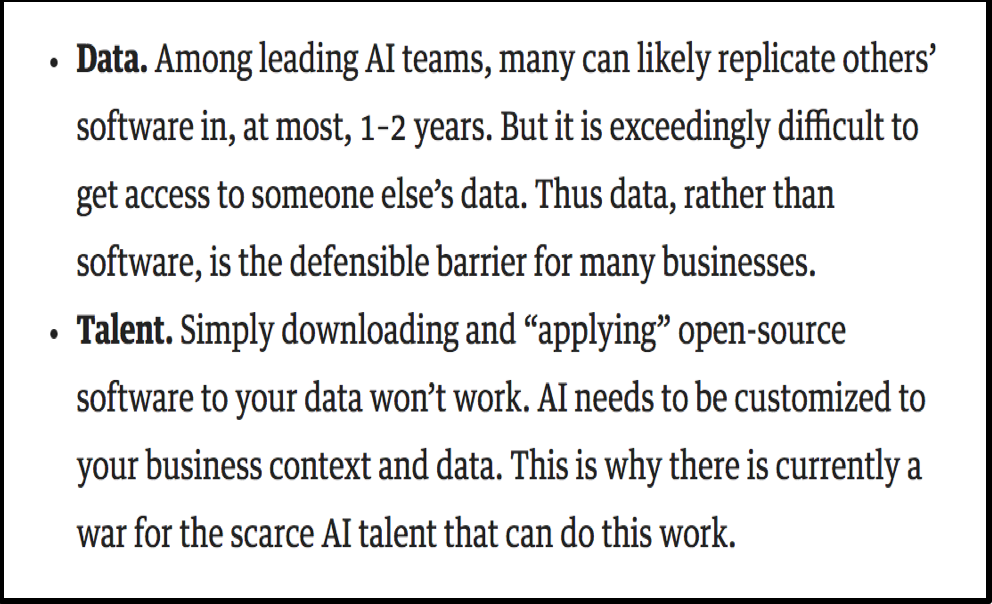
\includegraphics[scale=0.6] {images/talent_data_an.png}}
\caption{Andrew Ng on Data and Talent for Machine Learning. See \\
\url{https://hbr.org/2016/11/what-artificial-intelligence-can-and-cant-do-right-now}}
\label{fig:talent_and_data}
\end{figure}

\section{Trends} 
\label{sec:trends}
The main trends from the ONS can be summarized as follows: Ten plus years since the inception of SDN and six years after the original NFV proposal \cite{nfv}, we are seeing fully viable deployments that are close to being 100 per cent compliant with the original NFV vision, and we should very soon see a number of operators claim 100 per cent standards compliance. 

\bigskip
\noindent
Much of this success has been due to both flexible the open source communities which have enabled NFV to develop quickly. However, we are now seeing that the complexity involved in the disaggregation that is implied by SDN and NFV requires additional intelligence to be viable. Not surprisingly, almost every vendor is marketing some form of "AI" to deal with what we can think of as \emph{disaggregation complexity}\footnote{Here "AI" really means an ad-hoc collection of machine learning techniques.}.


\begin{figure}
\center{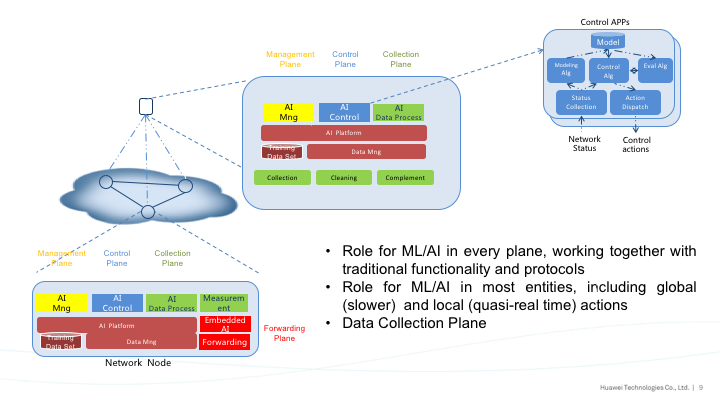
\includegraphics[scale=0.4, frame] {images/arch.png}}
\caption{Intelligence Network Infrastructure (INI) Architecture}
\label{fig:INI_architecture}
\end{figure}


\section{Stakeholder Meetings} 
\label{sec:stakeholders}
While I spoke with many people at the ONS, In general there were representatives from the major carriers as well as vendors and users at the event. I have summarized a few of the more interesting conversations I had with key stakeholders below. Nick McKeown is a professor at Stanford University and a founder and Chief Scientist at Barefoot Networks; you might remember Nick as one of the inventors of SDN. Axel  Clauberg is Vice President of Infrastructure at Deutsche Telekom. Michael Howard is an influential analyst at IHS Markit. Prodip Sen is CTO of NFV at HP Enterprise, Diego R. Lopez is a Senior Technology Expert at Telef\'onica, Don Clarke is a Principle Engineer at Cable Labs, and Dan Pitt is former Executive Director at the Open Networking Foundation. I summarize my discussions with each of them below. These discussions were similar to those held earlier at the Layer 123 event in The Hague. 

\begin{itemize}
\item \textbf{Nick McKeown} \\
I discussed the Intelligence Network Infrastructure (INI) concepts with Nick in some detail. See Figure \ref{fig:INI_architecture} for a schematic of the INI architecture. While he had a great deal of interest, we soon started talking about a project in which a Reinforcement Learning (RL) agent could learn a P4 program. I have an action item to pick that up with him in the near future.

\item \textbf{Axel  Clauberg} \\
I spoke with Axel for some time explaining the details of INI. He has little background in the kinds of mathematics required for successful deployment of machine learning applications at scale (see Figure \ref{fig:talent_and_data}). He outlined how DT, while at the forefront of automating NFV SDN environments, has great need for ML talent (apparently they have few people who can even think about these problems). I agreed to send Axel an email so that we can begin a more substantive discussion about INI and how it can help DT. The call is not yet scheduled.


\item \textbf{Michael Howard} \\
Michael is a respected analyst who focuses on emerging technologies for carriers. We discussed INI in detail, and he wants to interview me for a deeper dive on the topic of Huawei's ML and AI initiatives. This has not been scheduled. Note here: To this end (what is the larger Huawei vision for ML/AI) I am trying to get in touch with the Huawei ML and AI teams. However, we haven't yet found a way to make this happen.

\item \textbf{Prodip Sen} \\
Prodip is CTO of NFV Technologies at Hewlett Packard Enterprise (HPE). As such he is very much interested in standardized ML tools to further automate NFV implementations. While very interested in Huawei INI, he also has very little background in ML and hence the technical aspects of the solution are less compelling. \emph{This suggests that we need a marketing level presentation for people like Prodip}. In any event I took an action item to contact help for a discussion on the fundamentals of ML and how INI can help automate NFV deployments, as well as making them more "predictive".

\item \textbf{Diego R. Lopez} \\
I have known Diego for many years and we have worked on many projects together. In this discussion we talked
about the ideas behind the INI architecture, and of course, he was very interested. Telef\'onica has several AI/ML 
initiatives underway\footnote{Apparently including activities with Huawei, but I need to find more information about
exactly what the collaboration is.}, and there is excellent opportunity to further collaborate not only on use cases but
also on the underlying ML technology. We also had an interesting discussion about the role of \emph{causality} in ML and
beyond.

\item \textbf{Don Clarke} \\
Don was a principle at BT focusing on NFV before coming to CableLabs. He has extensive experience in what I would call "old school" automation techniques such as template driven automation (Puppet/Chef, Ansible, etc).  As such, he is very interested in what INI can bring to SDN (and NFV)  both in terms of automation and new capabilities (for example, predictive congestion avoidance).  We informally committed to further discussions. 

\item \textbf{Dan Pitt} \\
Dan and I discussed how to integrate INI into a more general SDN setting. In the months since the ONS, Dan has been working with others at Huawei on different projects.

\item \textbf{Network Engineers} \\
I spent quite a bit of time discussing the application of ML and causal reasoning systems to the networking domain. This was quite enlightening but one of the difficulties remains skill sets: network engineers
in general don't have the mathematical skills required for a deeper understanding of what is happening in ML and causal systems.

\end{itemize}


\section{My Talk} 
\label{sec:my_talk}
Like the event in The Hague and The NGP Forum, I talked primarily AI/ML, causality, and the Intelligent Network Infrastructure concept. While I believe that at some high level the audience understood the concept, the details were clearly beyond most participants. This again suggests that we need a more \emph{marketing oriented} talk/speaker for some parts of events like this. 

\begin{figure} [h!]
\center{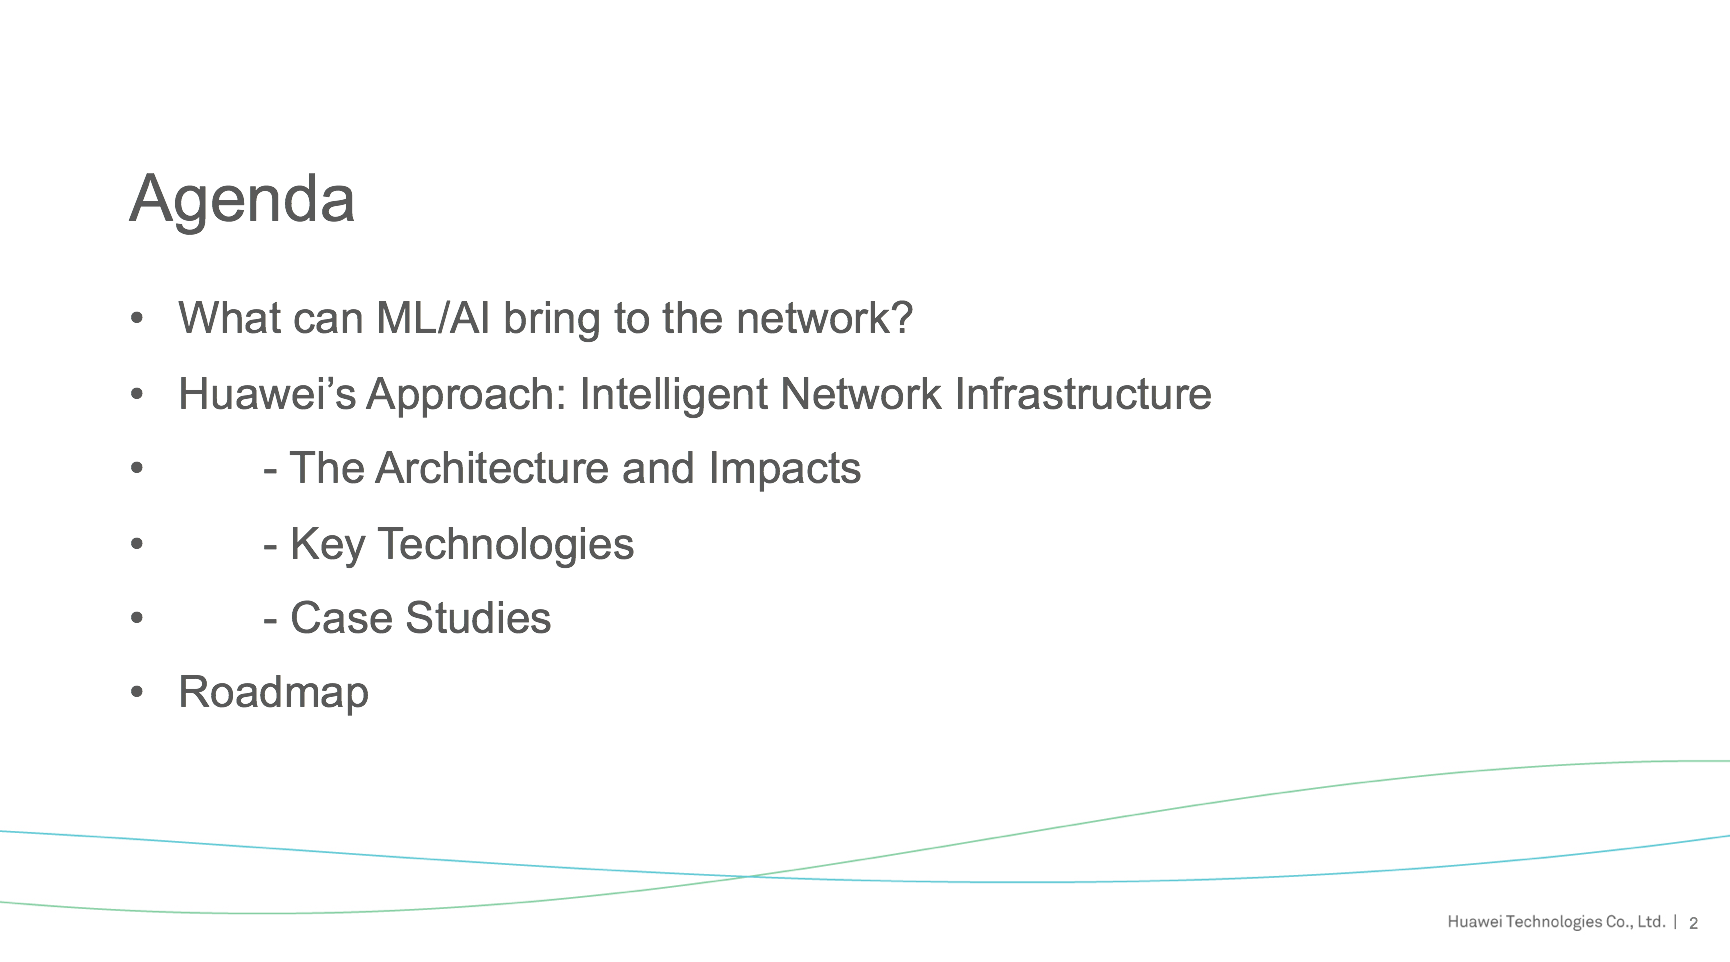
\includegraphics[scale=0.4, frame] {images/agenda.png}}
\caption{Agenda}
\label{fig:agenda}
\end{figure}


\bigskip
\noindent
I talked primarily about four of the INI use cases. The agenda can be seen in Figure \ref{fig:agenda}.  The first use case I talked about was Intelligent Traffic Balancing 
using an \emph{actor-critic} architecture for Reinforcement Learning\cite{Sutton:1998:IRL:551283,Lillicrap:2015aa}).  See Figure \ref{fig:intelligent_traffic_balancing}.

\begin{figure} [t]
\center{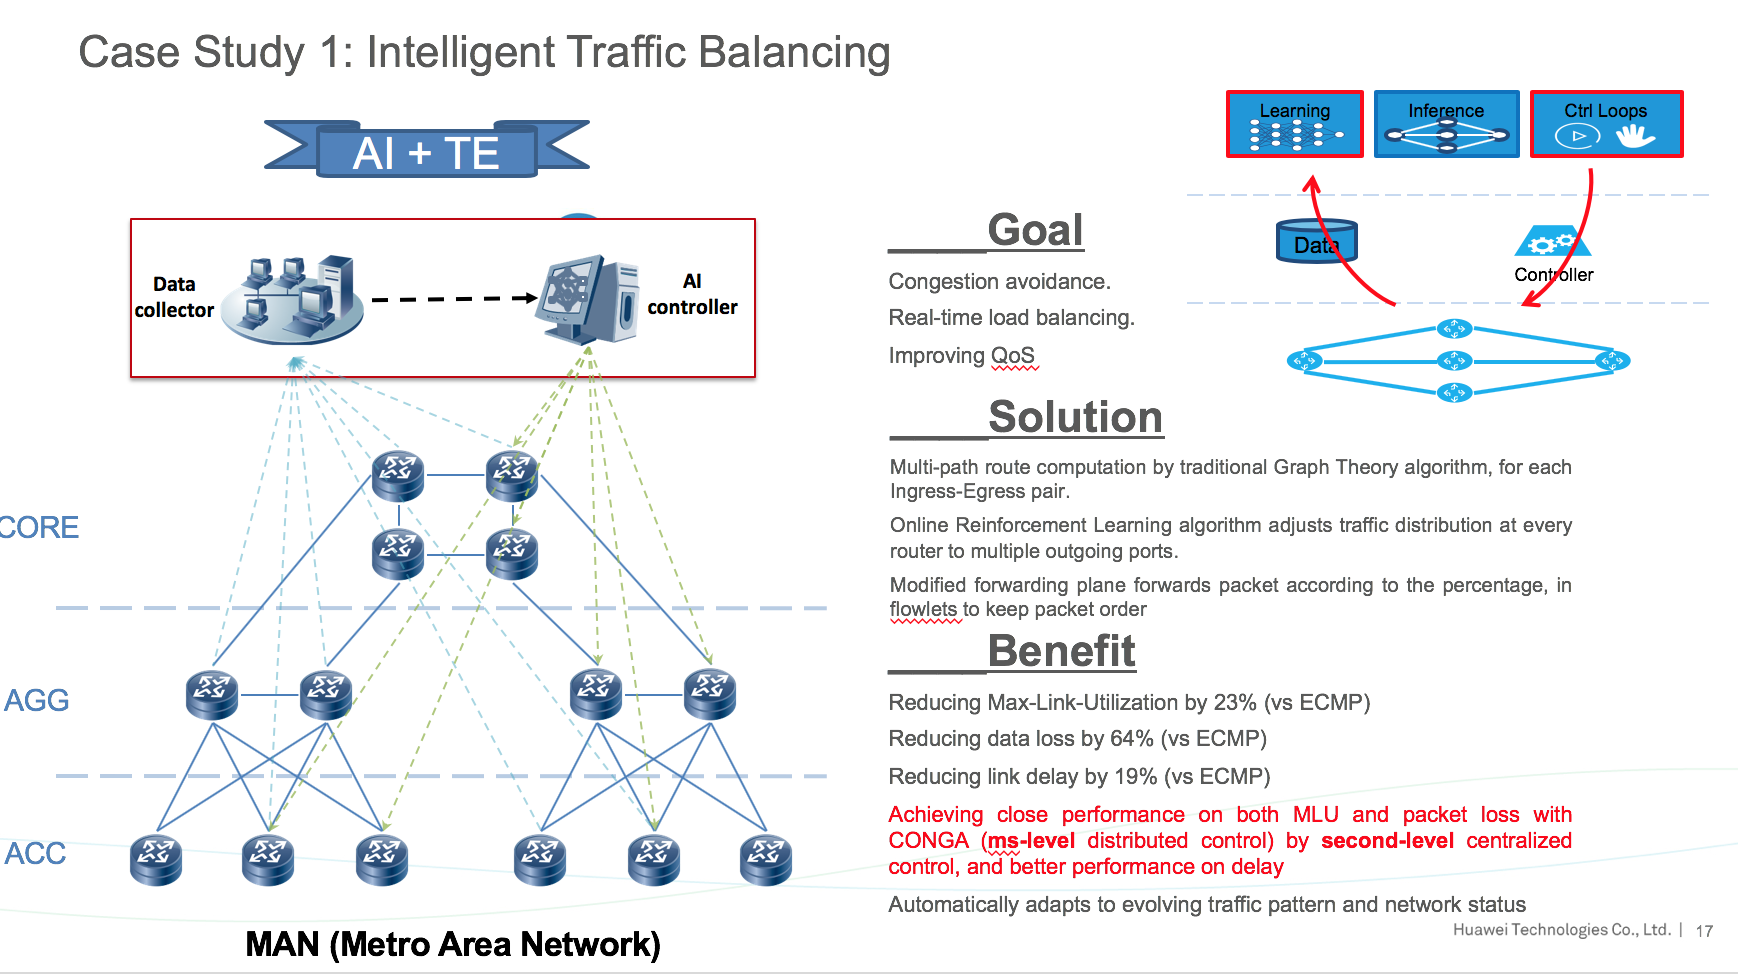
\includegraphics[scale=0.4, frame] {images/case_study_1_intelligent_traffic_balancing.png}}
\caption{Intelligent Traffic Balancing}
\label{fig:intelligent_traffic_balancing}
\end{figure}

\bigskip
\noindent
The first use case I talked about was Intelligent Traffic Balancing 
using an \emph{actor-critic} architecture for Reinforcement Learning\cite{Sutton:1998:IRL:551283,Lillicrap:2015aa}).  See Figure \ref{fig:intelligent_traffic_balancing}.

\bigskip
\noindent
The basic actor-critc architecture is shown in Figure \ref{fig:ac_architecture}. The second use case was Intelligent Overlay Routing, showing in Figure \ref{fig:intelligent_overlay_routing}.
The third use case was QoS Inferencing/SLA/QoS maintenance (using Conditional Variational Auto-Encoders, or CVAEs \cite{NIPS2015_5775}. 
See Figure \ref{fig:intelligent_overlay_routing}. Finally, I talked a bit about  Intelligent Measurement (Figure \ref{fig:intelligent_measurement}). There was significant interest in 
all four use cases; however, in both cases the actual details of how 
RL or CVAEs work was  really beyond the audience's ability to absorb in the time allotted, which again makes me suggest that a more marketing-oriented approach might have 
been more appropriate for the venue. 

\begin{figure}
\center{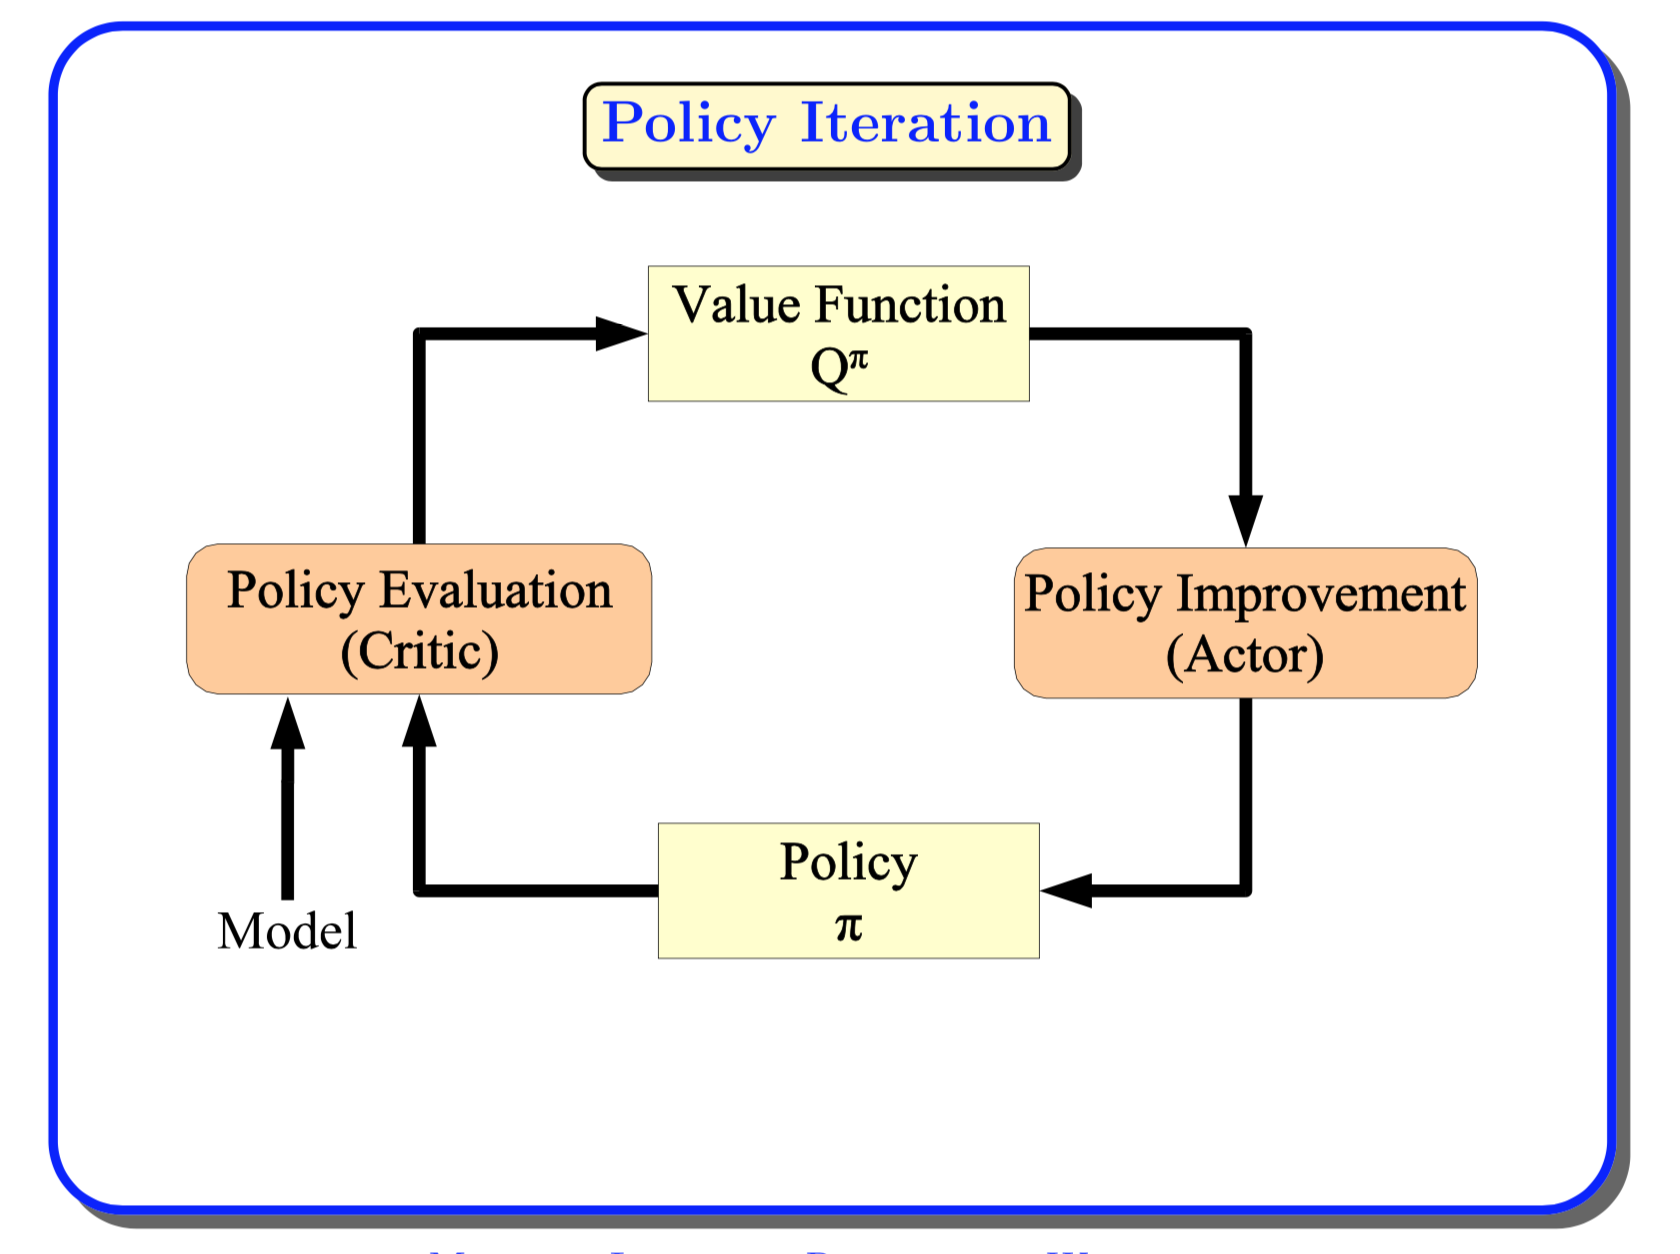
\includegraphics[scale=0.4] {images/ac_architecture.png}}
\caption{Basic Actor-Critic Architecture}
\label{fig:ac_architecture}
\end{figure}



\section{Conclusions and Recommendations} 
\label{sec:conclusions}
There are several takeaways from this meeting. First, the meeting is clearly a worthwhile forum to meet and interact with industry leaders. However (and again, similar to the Layer 123 event),
this interaction appears to be primarily on the marketing or "C-level" (executive level), where the actual details of the technologies being discussed are less useful. Again, a more \emph{marketing oriented} approach may be more effective here, especially for technologies like ML which mathematical in nature and hence perhaps more difficult to understand (at least at that level). 

\begin{figure} [t]
\center{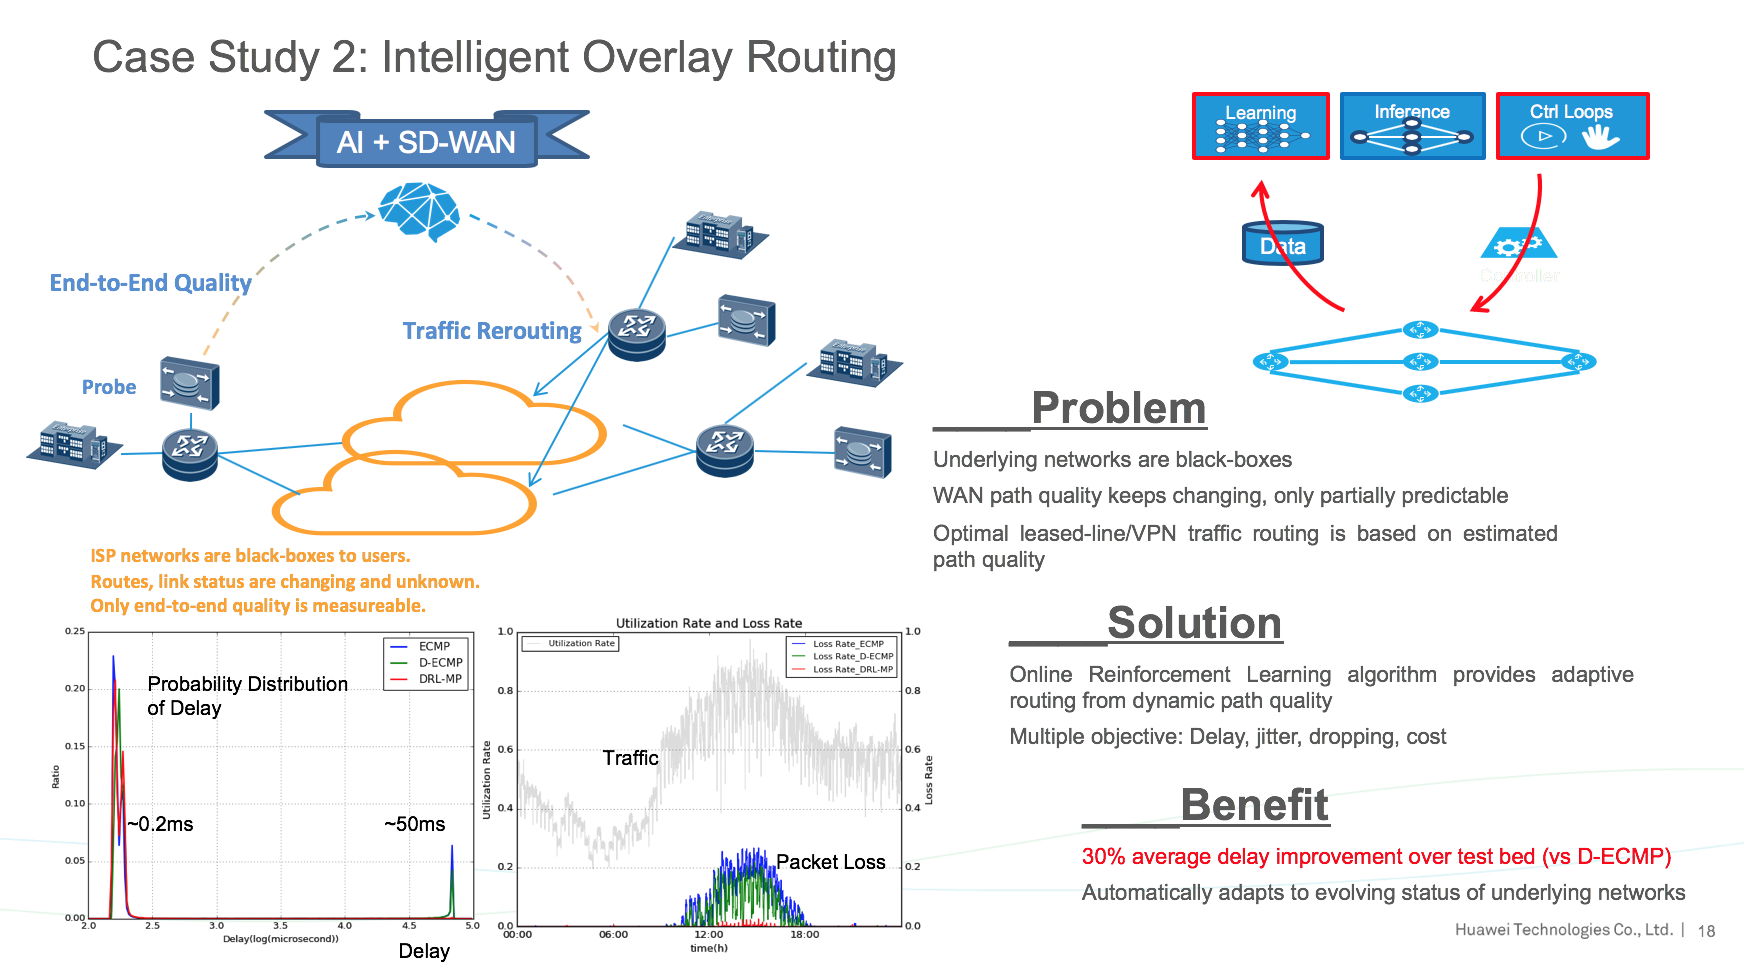
\includegraphics[scale=0.4, frame] {images/case_study_2_intelligent_overlay_routing.png}}
\caption{Intelligent Overlay Routing}
\label{fig:intelligent_overlay_routing}
\end{figure}


\begin{figure} [t]
\center{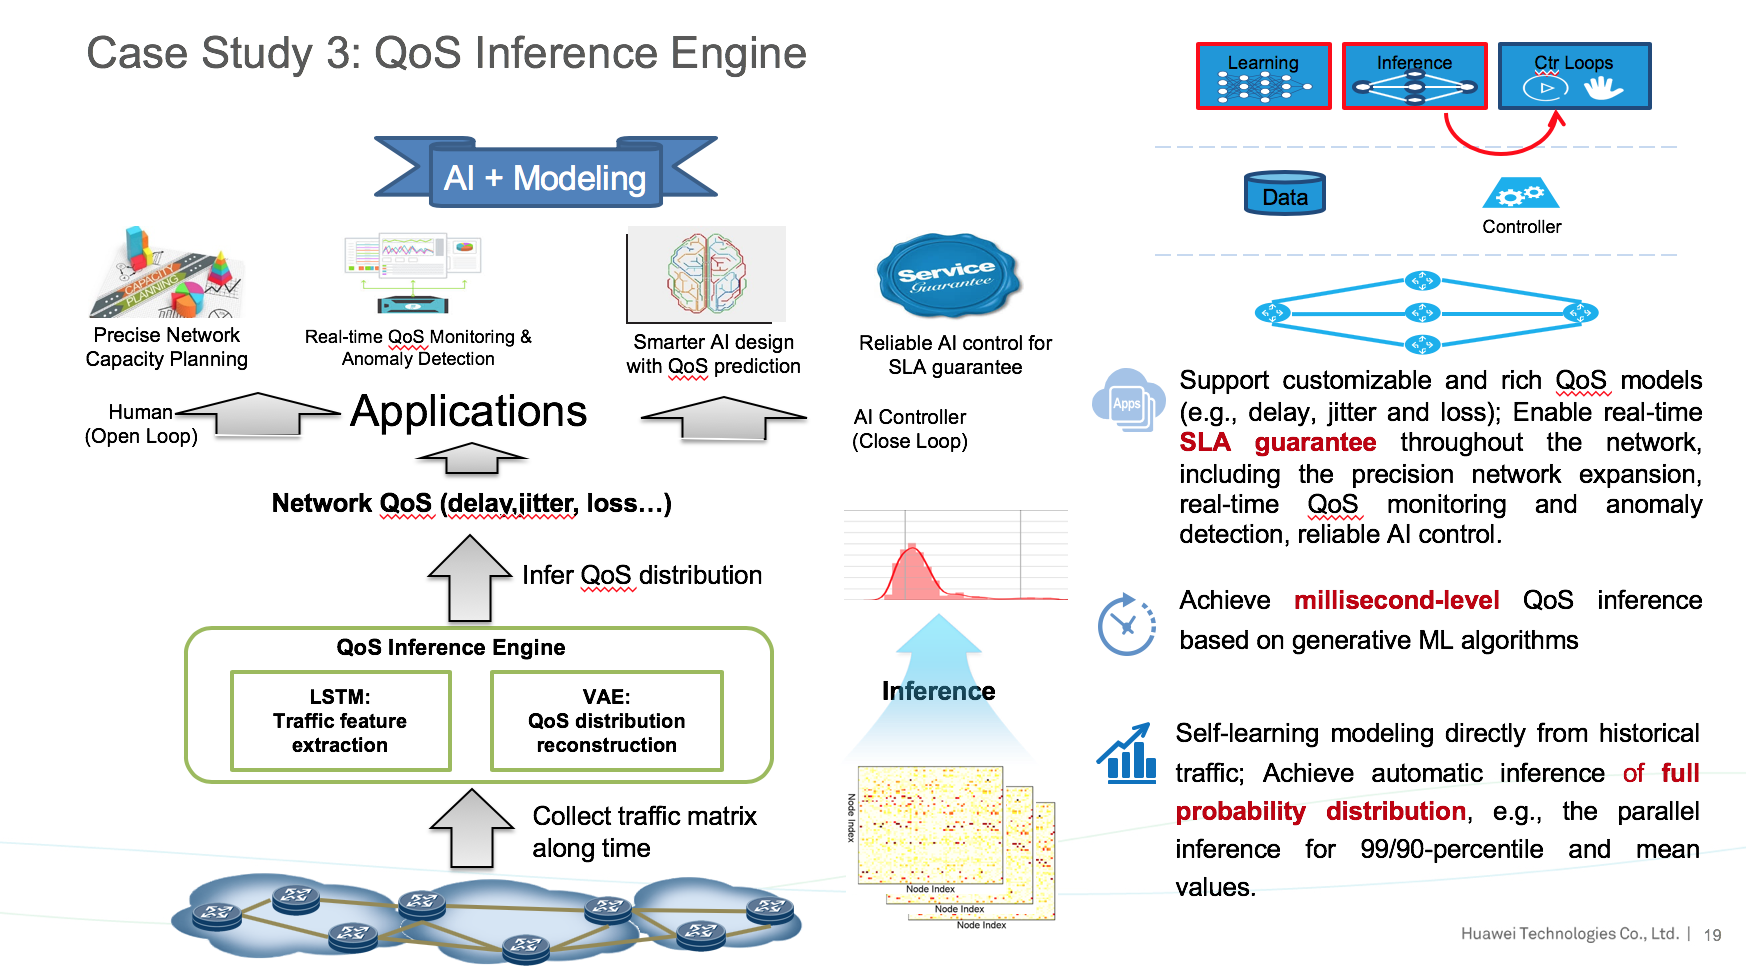
\includegraphics[scale=0.4, frame] {images/case_study_3_qos_inference_engine.png}}
\caption{QoS Inference Engine}
\label{fig:qos_inference_engine}
\end{figure}

\begin{figure} 
\center{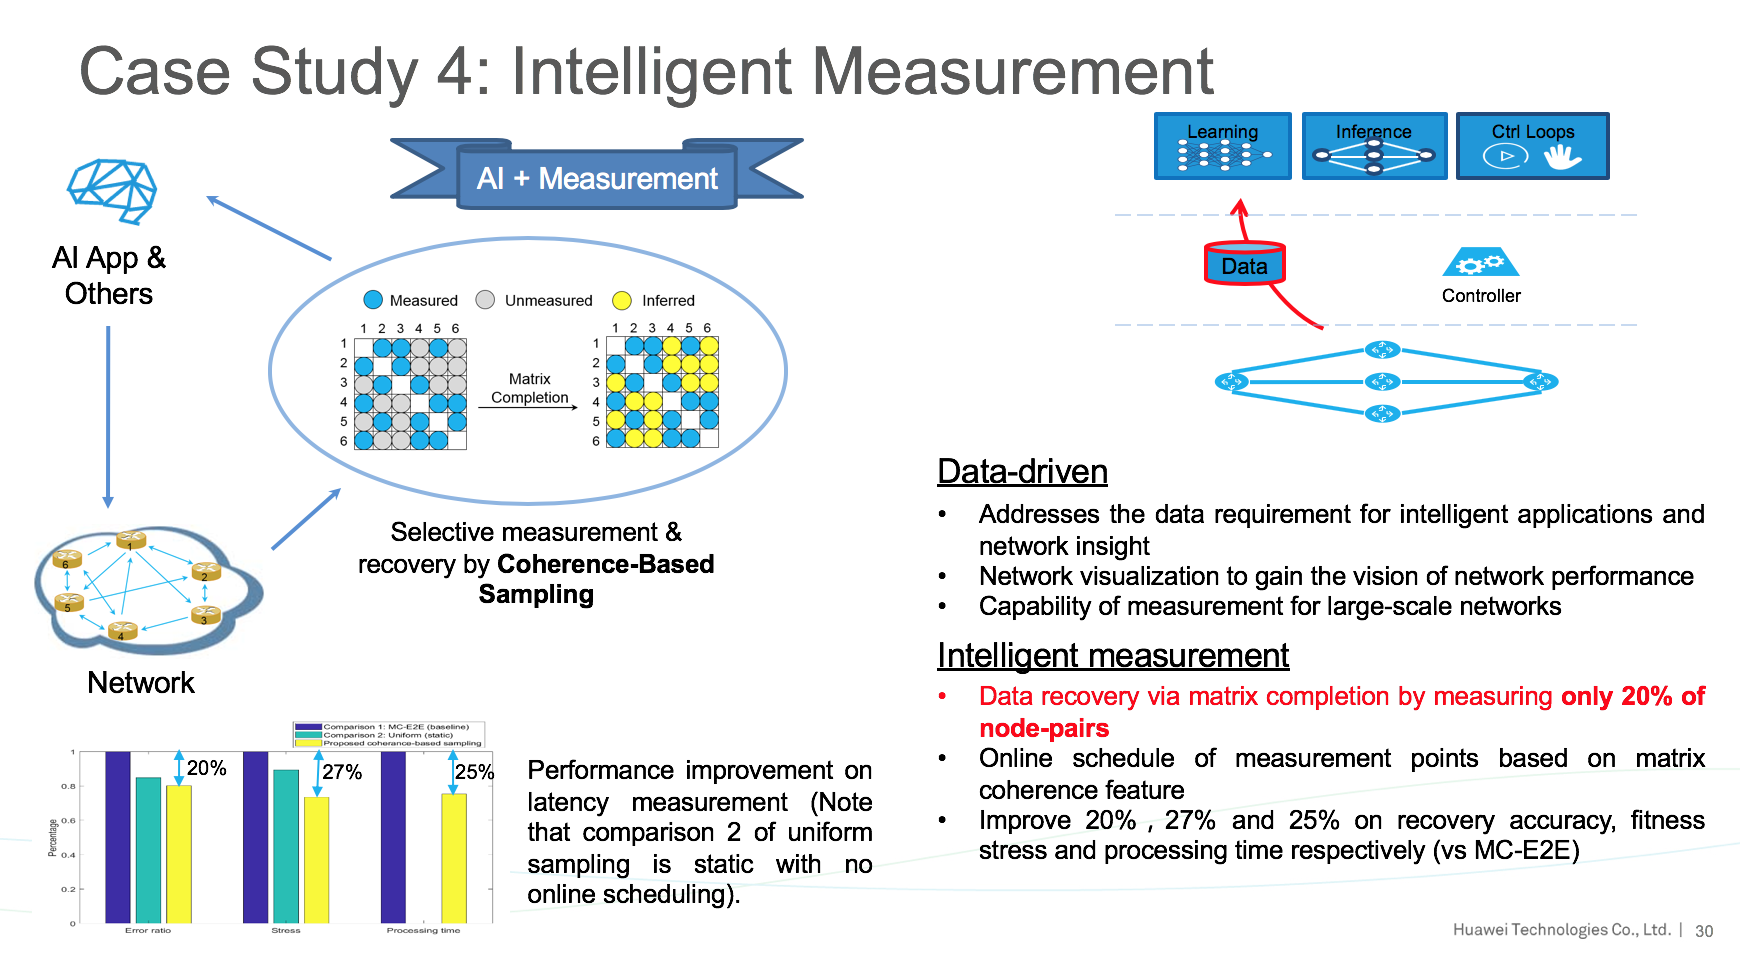
\includegraphics[scale=0.4, frame] {images/case_study_4_intelligent_measurement.png}}
\caption{Intelligent Measurement}
\label{fig:intelligent_measurement}
\end{figure}

\bigskip
\noindent
The main recommendations of this section can be summarized as follows: First, in the near term we need to provide more detail for the use cases, and to clearly explain the value proposition of each use case. This will also need to be publicized in various venues (see Section \ref{sec:recommendations} below), Second, we need a \emph{theory} of networking into which will unify these ad-hoc approaches; to put in more simply, ad-hoc application of ML techniques 
to the networking domain worn't work. Finally, we need to reach out to a cross-section of the 
management stack so that we can influence at all levels.

\subsection{Recommendations}
\label{sec:recommendations}
\begin{itemize}
\item \textbf{Provide more detail on what exactly INI is and what its capabilities are} \\
In particular,  we describe INI as a set of use cases, not a \emph{system} or \emph{platform}.  In particular,  how does INI work (this is essential as INI must be \emph{explainable} 
if it is to be adopted by service providers), how does INI solve existing and future use cases,
and how a theory of network is addressed by INI.

\item \textbf{Further develop and add to the INI use cases} \\
The the four INI use cases, listed below, need more detail and easy-to-understand examples. The proposed use cases for INI include:

\begin{figure}
\center{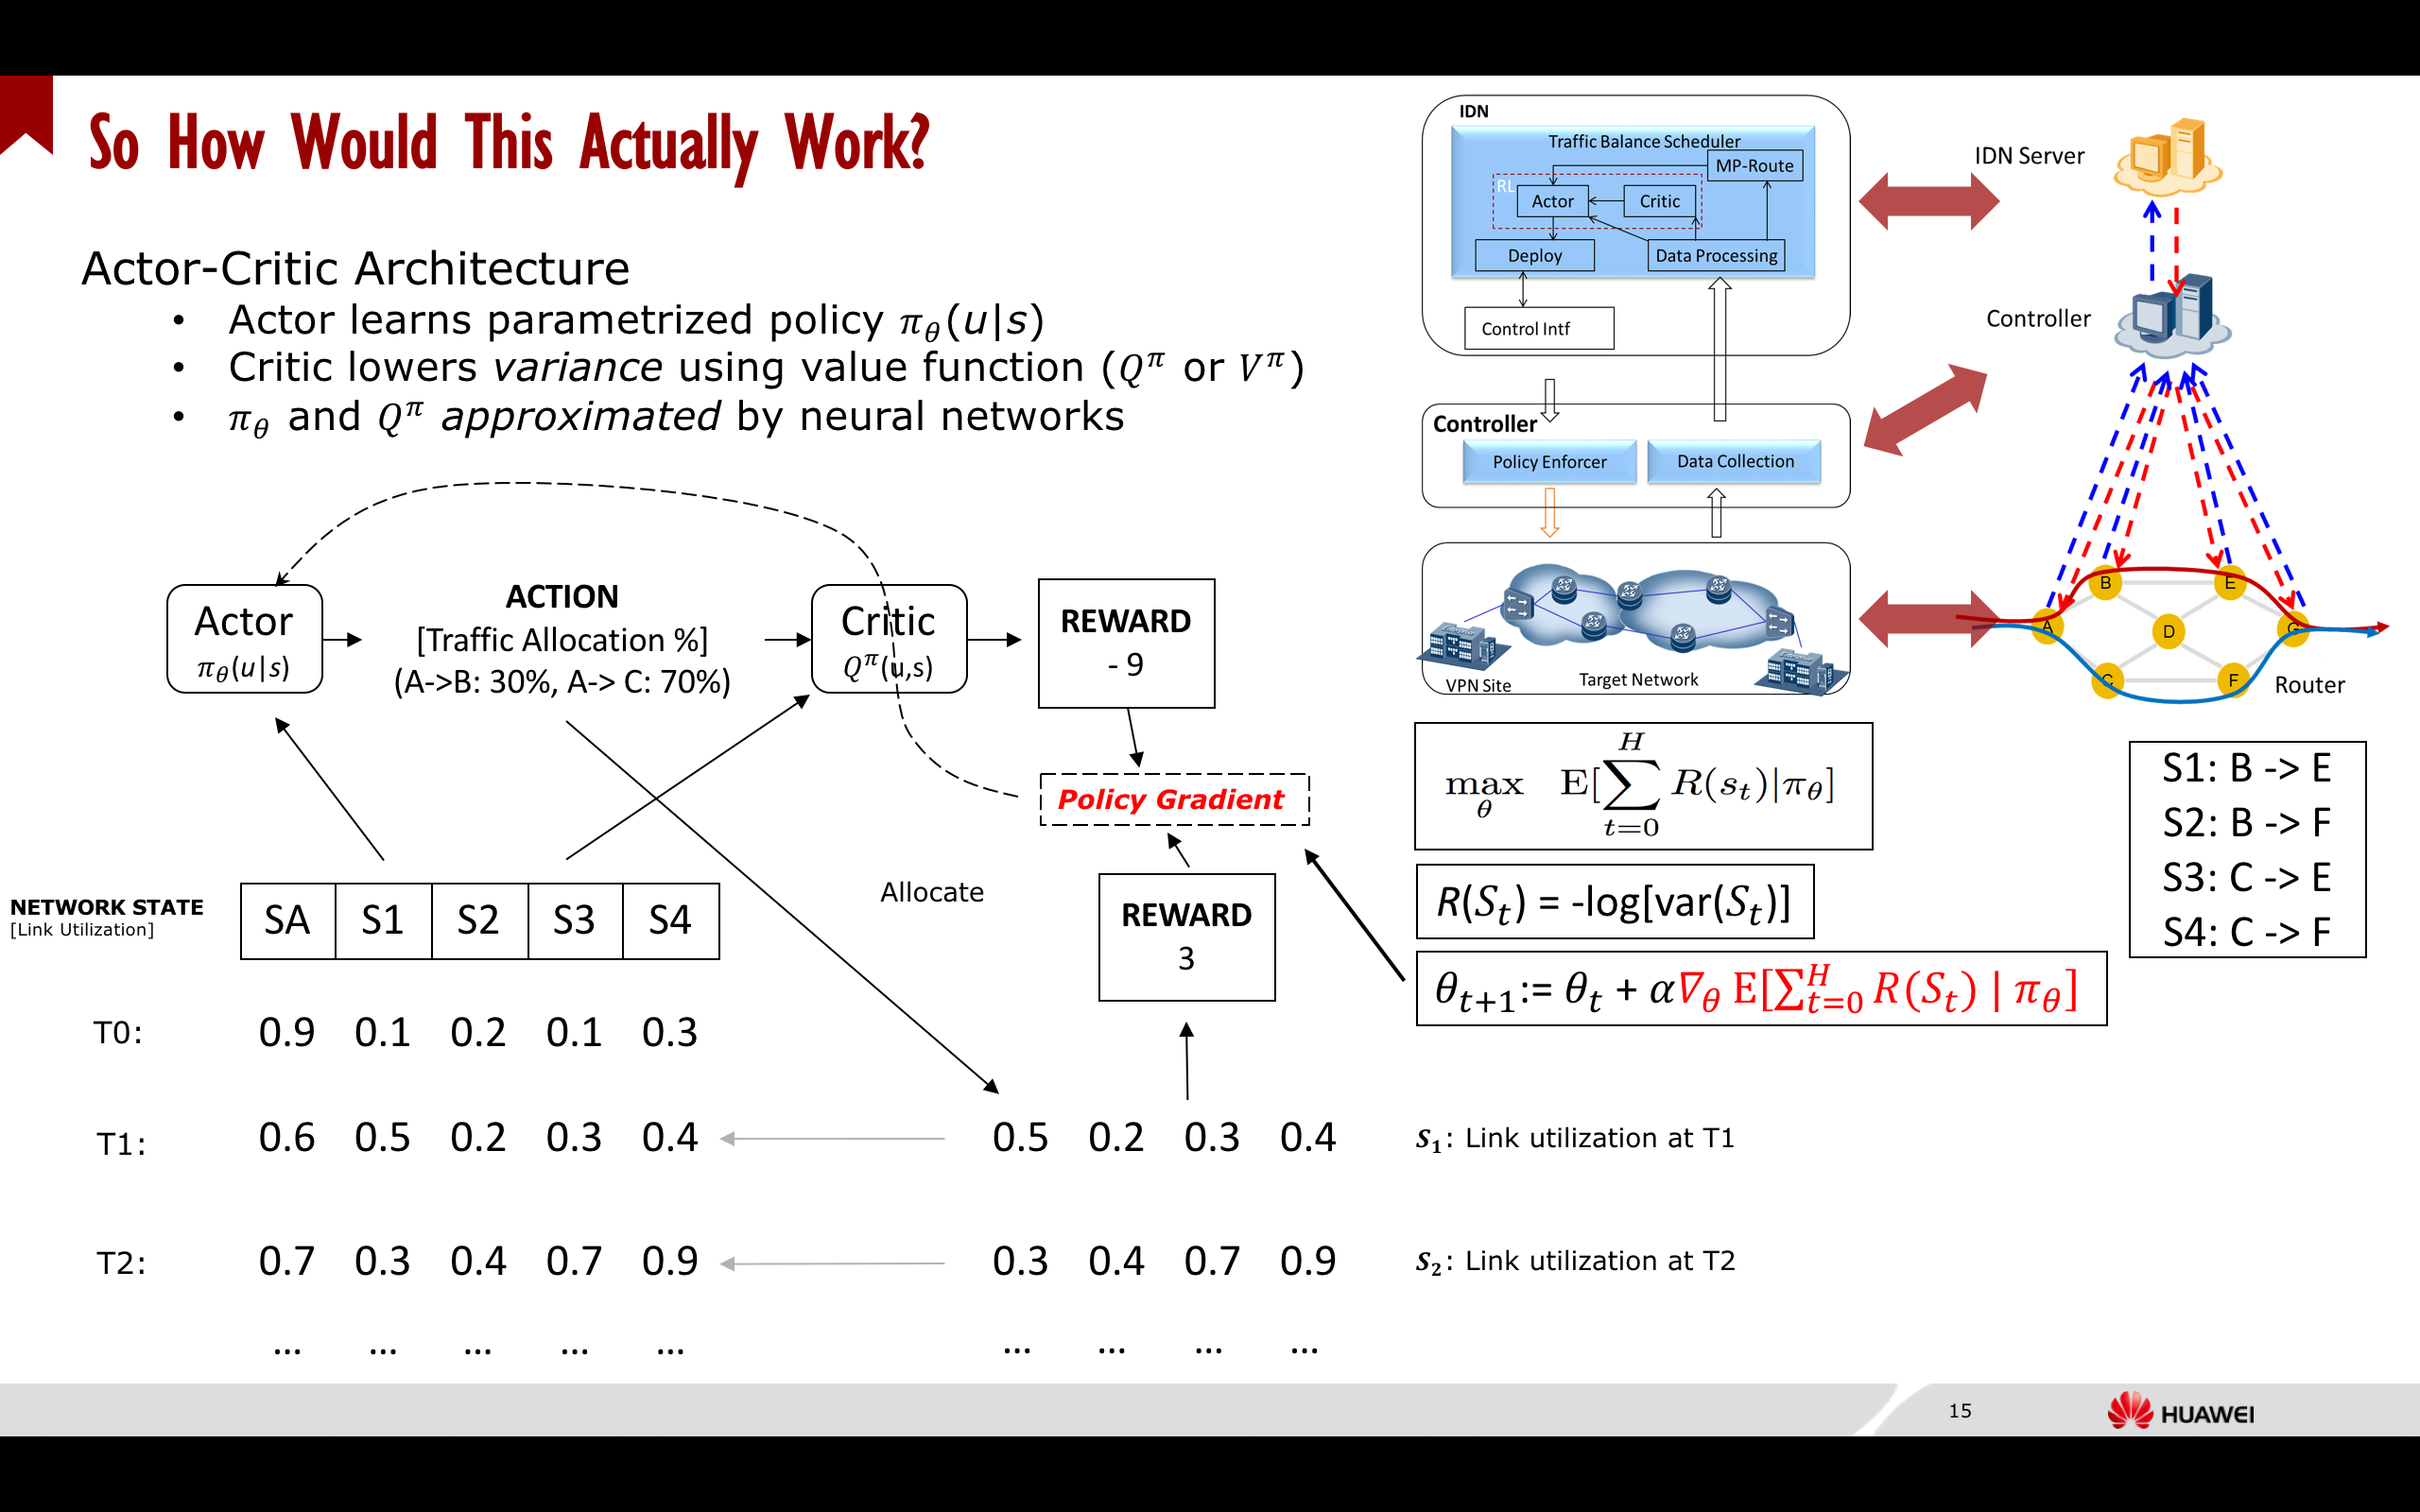
\includegraphics[scale=0.3] {images/ac.png}}
\caption{Actor-Critic Architecture for the Traffic Balancing Use Case}
\label{fig:ac}
\end{figure}

\begin{itemize}
\item Intelligent Traffic Balancing
\item Intelligent Overlay Routing
\item QoS Inference
\item Intelligent Measurement
\end{itemize}

\bigskip
\noindent
In addition to these use cases, we need to show how INI is \emph{extensibile} to new use cases; such use cases could be, for example, from the 5G, NFV, AR/VR. and 
other domains.

\item \textbf{Flesh out the \emph{theory} of Network Intelligence} \\
Most of the "ML for Networking" approaches we see in the market are \emph{ad-hoc} application of known ML techniques to the networking domain. However, there is no unifying theory (or idea) of a network actually is. The work I'm doing with John Doyle\footnote{See \url{http://www.cds.caltech.edu/~doyle/}} at CalTech is intended to fill this gap. We will publish results of integrated control plus learning environments for networking as soon as possible.


\item \textbf{Connect to other ML work in the networking area} \\
There is quite a bit of older work on using ML to solve various problem in the networking space (see, for example  \cite{Tao:2001aa}), 
and with all of the current interest in ML for networking we're seeing new work that attempts to leverage current advancements 
in ML\footnote{See, for example, \cite{Stampa:2017aa}.}.  However, all of this work suffers from the lack of \emph{theory} that I mention above. This theory will need to not only address the fundamental nature of networking but also integrate with ideas of fast and slow control and machine learning. As mentioned above, this theory is the focus of work I am doing with John Doyle at CalTech. This also implies that network engineers must also become facile with machine learning mathematics, concepts, and
implementation.

\item \textbf{Create materials for different groups} 
Different groups require different levels of explanation of both the technology and the associated use cases. These groups include
\begin{itemize}
\item{C-Level}
\item{Network Engineers}
\item{Marketing}
\end{itemize}
Clearly each of these categories require a different level of presentation and different presentation skills. We should develop a set of presentations and presenters that can
address these different categories

\item \textbf{Present INI at more venues} \\
These should include not only the typical networking venues (IETF, Layer123, etc) but also to machine learning (e.g., NIPS, ICLR, etc)  and control conferences. These later conference types are of great 
importance as we want to establish leadership in though and innovation.

\item \textbf{Contribute data, source code, and models to public repositories (github)} \\
Huawei should develop guidelines for the release and open-souring of prototype code, data, and models to our github\footnote{\url{https://github.com/}} repositories. 
Along with these guidelines, we should have a clear governance model and implementation for what goes into our
public repositories, who can modify these repositories, etc.
\end{itemize}

\bigskip
\noindent
Finally, we need to create deeper connections between the Future Network Theory Laboratory and the work being done in other 
parts of the company in both control and machine learning. For example, we would like to have results in the areas of both control
and learning theory for networking. We also need to get this work into the public as soon
as we have solid results, both in terms of conferences and in public repositories (again, for example \url{https://github.com}).  
To that end I have begun to seek out the appropriate people to facilitate these interactions.

\begin{figure}[b]
\center{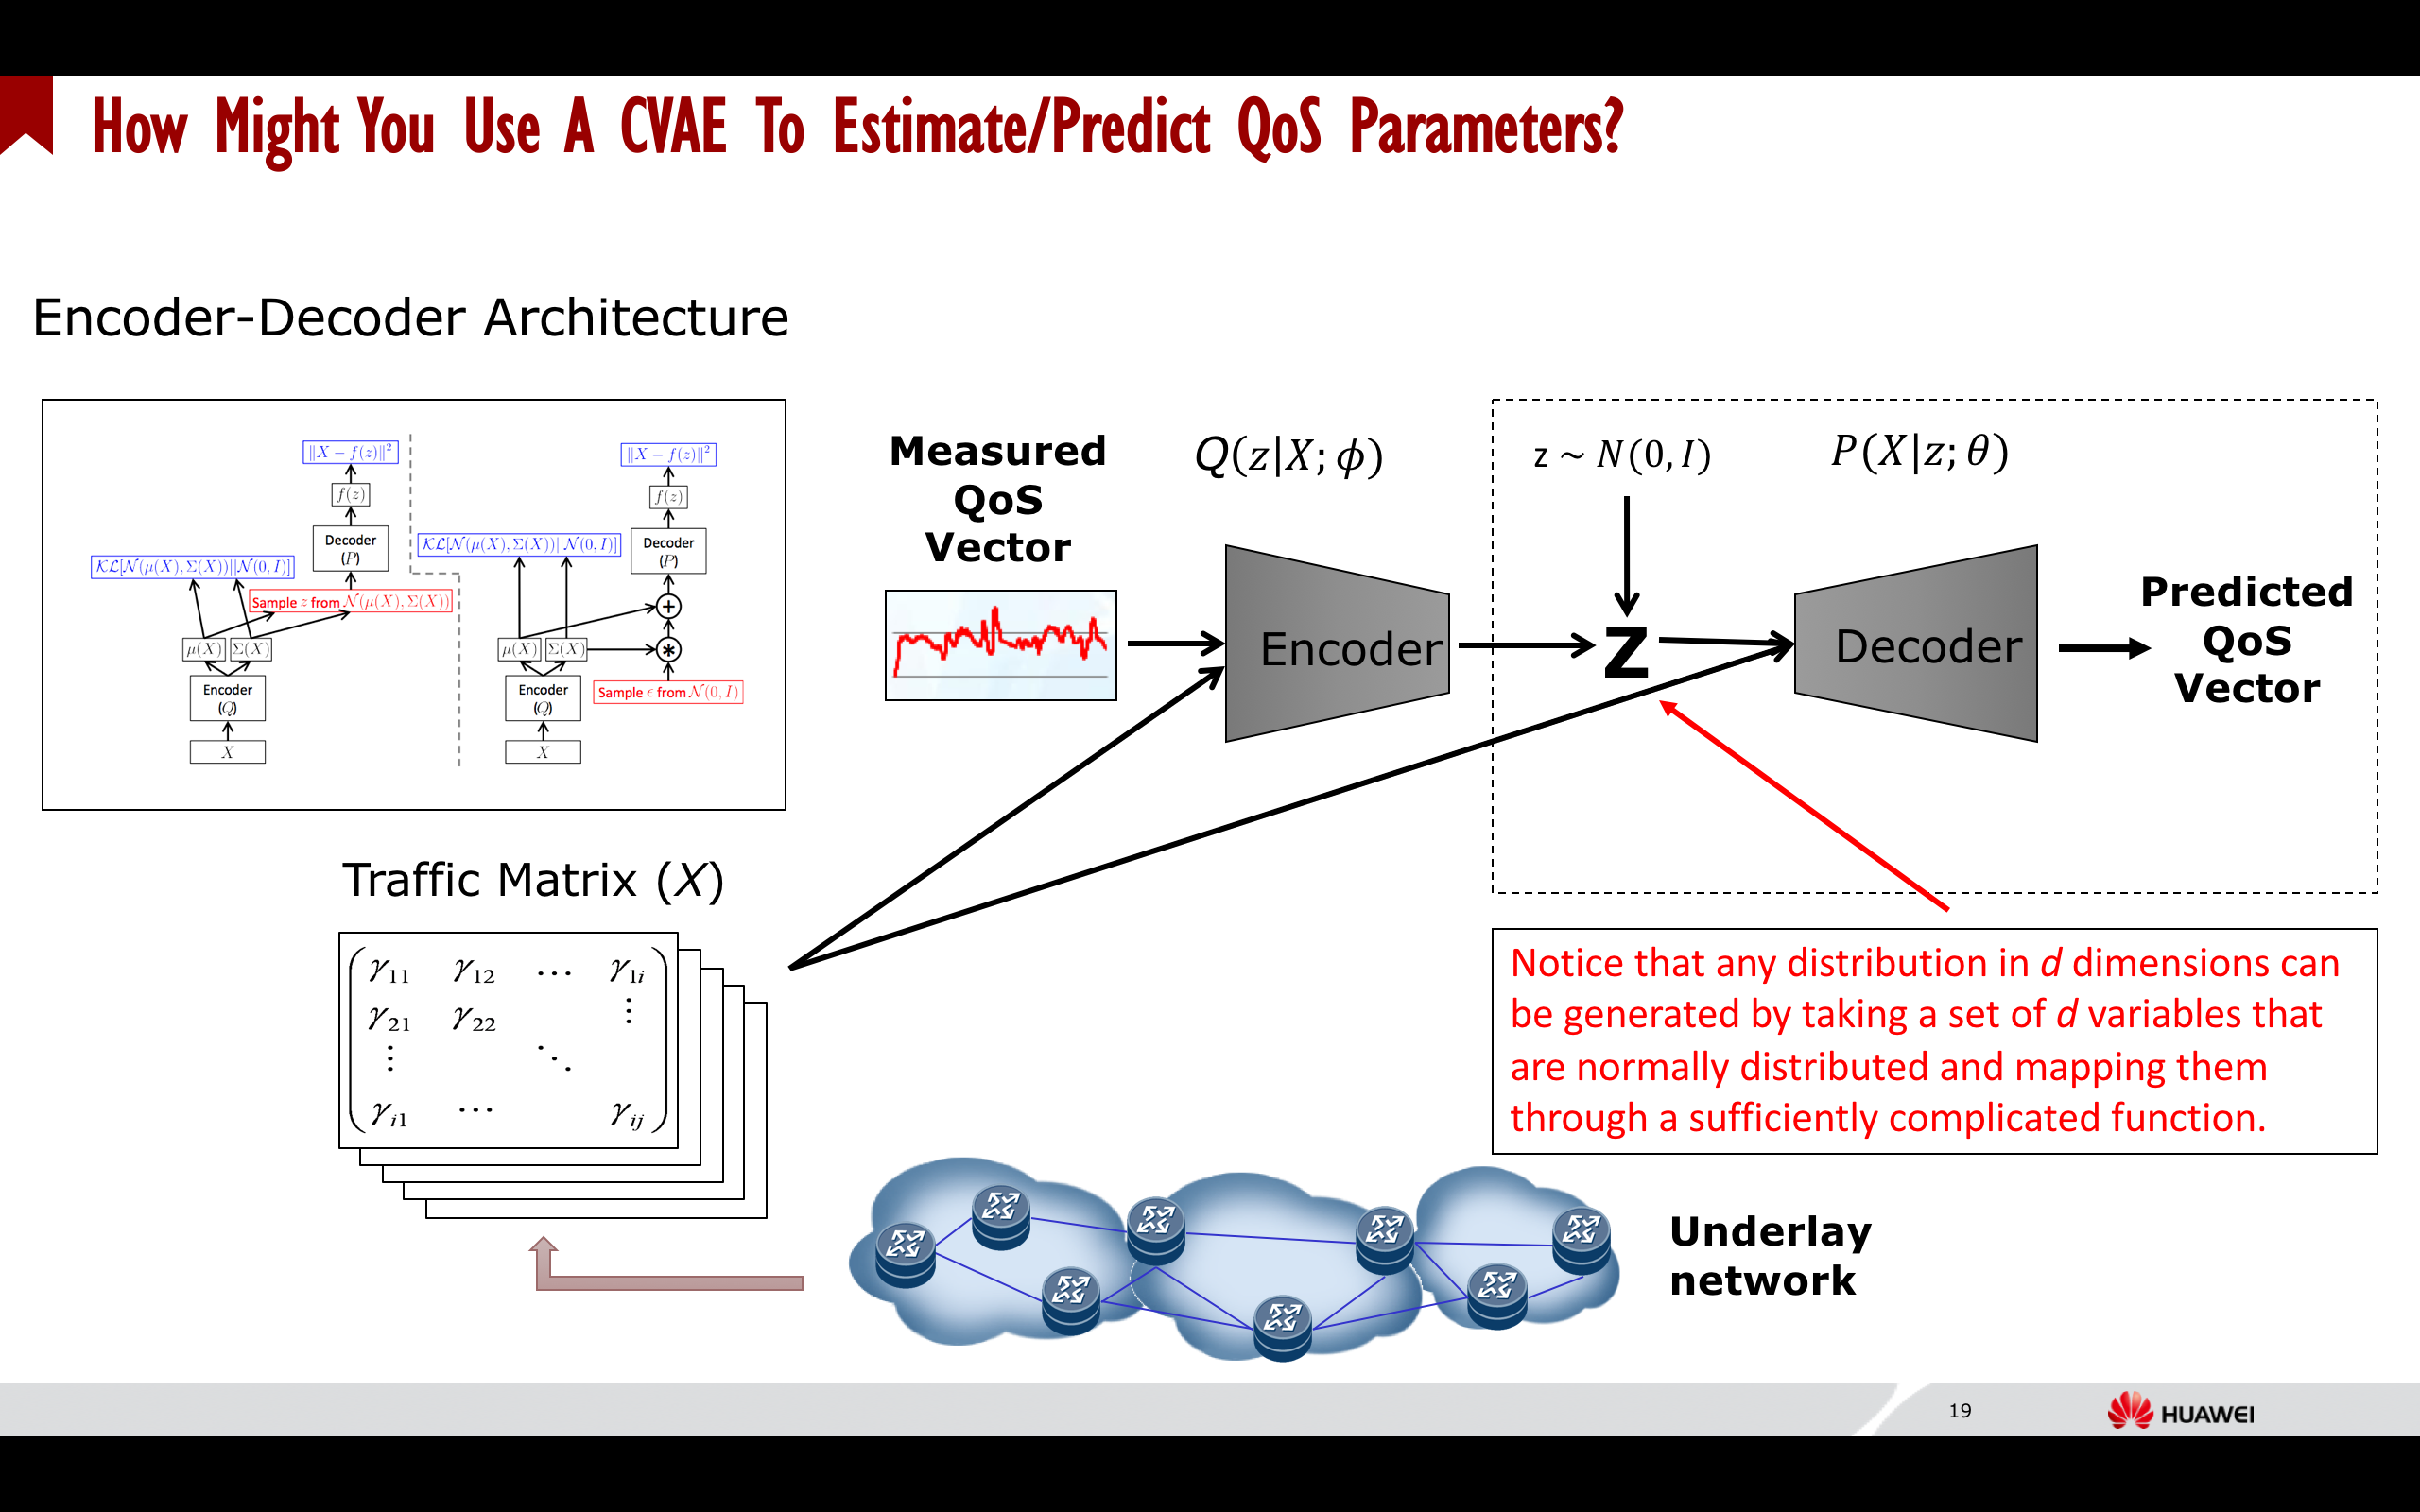
\includegraphics[scale=0.3] {images/cvae.png}}
\caption{Conditional Variational AutoEncoder (CVAE) for the QoS/SLA Use Case}
\label{fig:cvae}
\end{figure}

\newpage
\bibliographystyle{ieeetr}
\bibliography{/Users/dmm/papers/huawei/bib/huawei.bib}



\end{document} 
